\section{Results and Discussion}
\label{sec:results}

This section presents the thermal response of the Gyroid TPMS/PCM composite under three heating power levels (10~W, 20~W, 30~W), analyzing the temperature evolution, spatial stratification, and power-dependent behavior.

\paragraph{Temperature evolution.}
Fig.~\ref{fig:temp_curves} presents the temperature evolution curves for the Gyroid TPMS/PCM composite at three heating powers. Three distinct thermal regimes are evident across all power levels: (i)~an initial sensible heating phase where all temperatures rise approximately linearly from ambient; (ii)~a phase transition plateau near 42\textdegree C where the temperature rise slows as latent heat is absorbed; and (iii)~a post-melting sensible heating phase where temperatures rise again in the liquid state. The 42\textdegree C phase change temperature is indicated by the horizontal dashed line.

\begin{figure}[htbp]
\centering
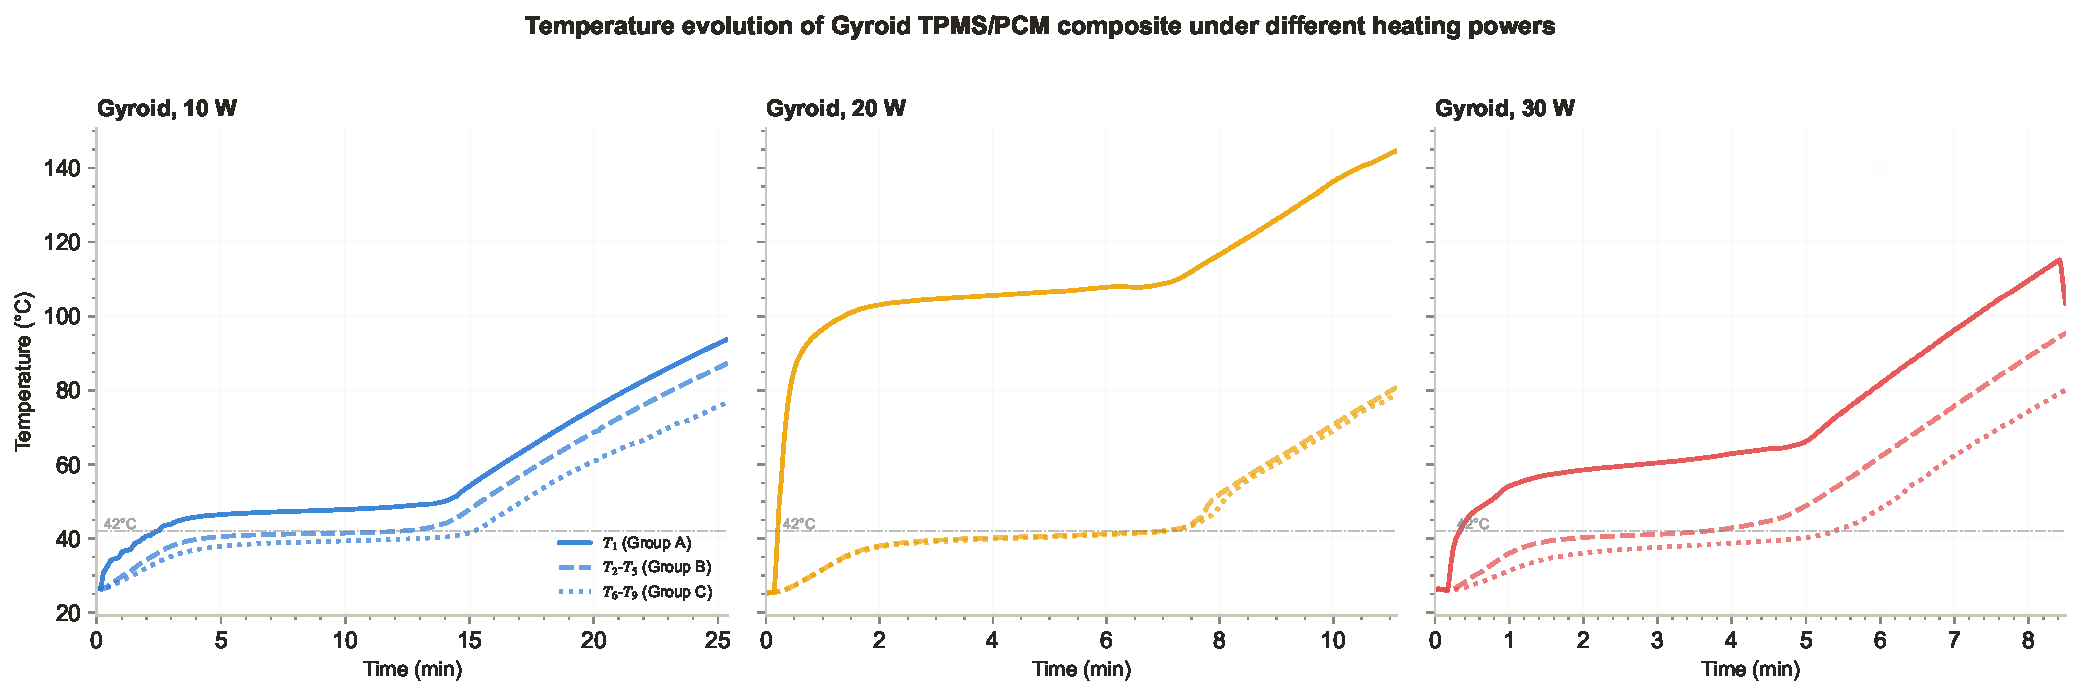
\includegraphics[width=\linewidth]{figures/fig_01_temperature_curves.pdf}
\caption{Temperature evolution of Gyroid TPMS/PCM composite under (a)~10~W, (b)~20~W, and (c)~30~W heating power. Three groups are shown: Group~A ($T_1$, solid), Group~B ($T_2$--$T_5$ mean, dashed), and Group~C ($T_6$--$T_9$ mean, dotted). The horizontal dash-dotted line indicates the PCM phase change temperature (42\textdegree C).}
\label{fig:temp_curves}
\end{figure}

At 10~W (Fig.~\ref{fig:temp_curves}a), the extended duration (25.4~min) allows clear observation of the phase change plateau, particularly in Groups B and C where the temperature remains near 42\textdegree C for approximately 5--8 minutes before rising again. Group~A ($T_1$), being closest to the heater, shows a less pronounced plateau as it reaches higher temperatures more rapidly. At 20~W (Fig.~\ref{fig:temp_curves}b), the phase change plateau is compressed to approximately 3--4 minutes due to the higher heating rate, and Group~A reaches 144.7\textdegree C---well above the phase change temperature. At 30~W (Fig.~\ref{fig:temp_curves}c), the experiment duration is further reduced to 8.5~min, and the phase change plateau is barely discernible, indicating that the heating rate significantly exceeds the PCM's ability to absorb latent heat at this power level.

\paragraph{Spatial temperature stratification.}
A consistent temperature stratification pattern was observed across all power levels: $T_1 > T_{2\text{-}5} > T_{6\text{-}9}$. This radial thermal gradient reflects the heat flow direction from the central heater outward through the TPMS lattice/PCM composite. Such stratification patterns are consistent with convection-driven melting behavior reported for paraffin in enclosures and shell-and-tube systems~\cite{kamkari2014experimental,kirincic2021influence,kirincic2021ahe,khakpour2014natural}, where natural convection in the molten PCM redistributes heat toward the upper region of the melt and steepens the effective radial gradient. The temperature differences between groups provide insight into the effective thermal resistance of the composite at different radial positions.

Fig.~\ref{fig:comparison}a quantifies the final temperatures achieved by each group at each power level. At 10~W, the temperature spread between Groups A and C is 17.1\textdegree C (93.8 vs.\ 76.7\textdegree C), indicating moderate thermal gradients within the composite. At 20~W, the spread increases dramatically to 66.0\textdegree C (144.7 vs.\ 78.7\textdegree C), with Group~A reaching temperatures far exceeding the PCM phase change point while Groups B and C remain much closer to it. At 30~W, the spread is 23.4\textdegree C (103.5 vs.\ 80.1\textdegree C), suggesting that the shorter experiment duration limits the development of extreme thermal gradients.

\begin{figure}[htbp]
\centering
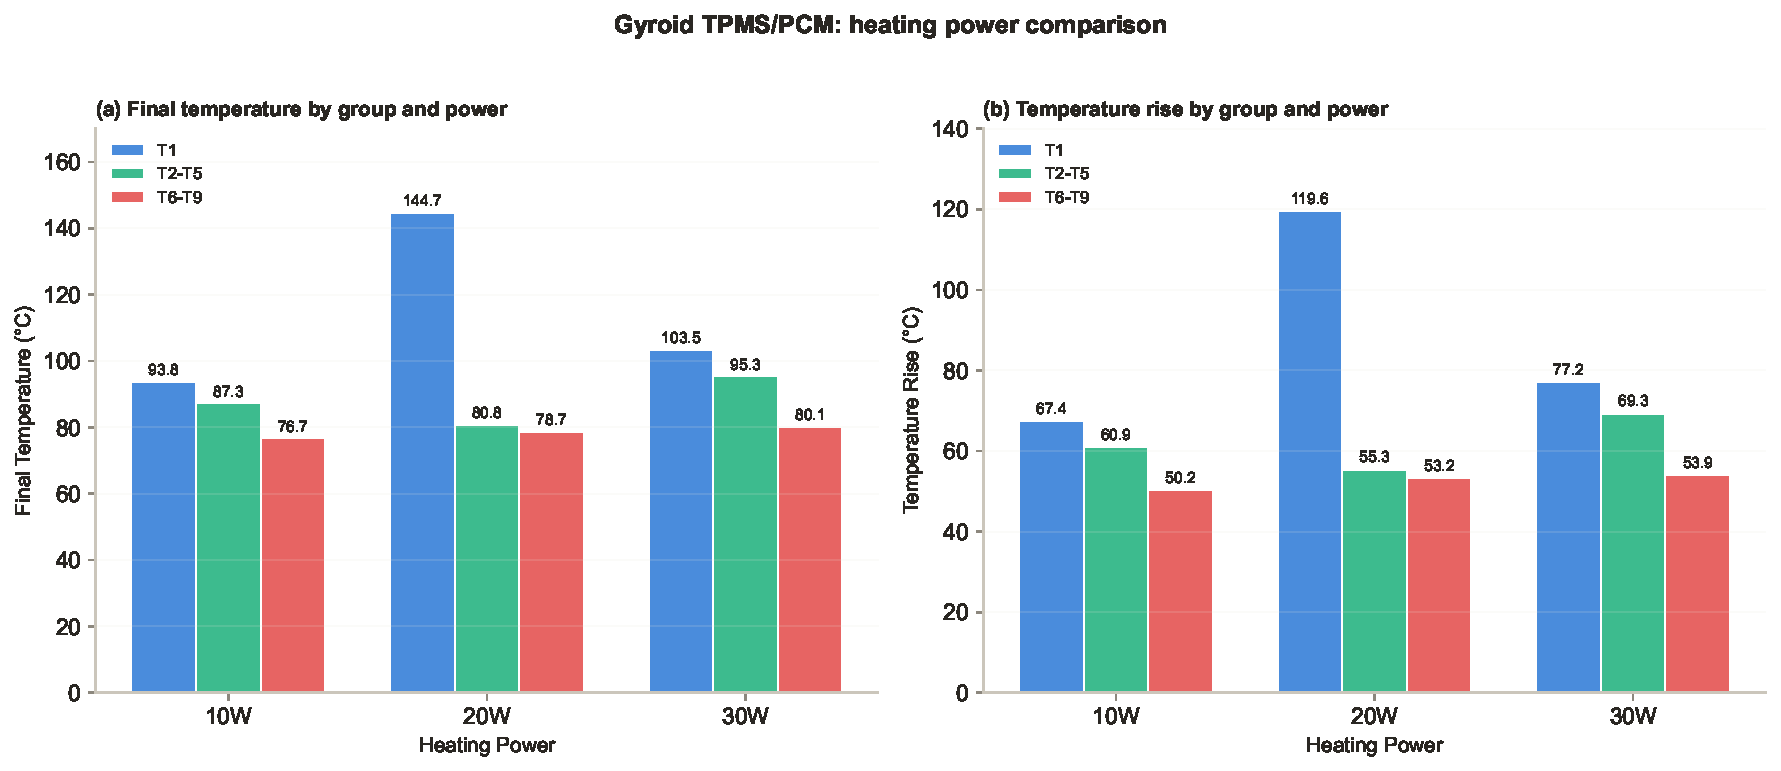
\includegraphics[width=\linewidth]{figures/fig_02_power_comparison.pdf}
\caption{(a)~Final temperatures and (b)~temperature rise by group and heating power for the Gyroid TPMS/PCM composite. Error in final temperature measurement: $\pm$0.1\textdegree C.}
\label{fig:comparison}
\end{figure}

\paragraph{Power-dependent behavior.}
Fig.~\ref{fig:comparison}b compares the temperature rise ($\Delta T = T_{\text{final}} - T_{\text{initial}}$) across power levels. For Group~A, the temperature rise increases from 67.5\textdegree C (10~W) to 119.5\textdegree C (20~W) to 77.2\textdegree C (30~W). The non-monotonic trend---with 20~W producing the highest temperature rise---reflects the interplay between heating power and experiment duration: at 20~W, the 11.1~min duration allows Group~A to accumulate substantial thermal energy, while at 30~W the shorter 8.5~min duration limits the total energy input despite the higher power.

For Groups B and C, the temperature rise shows a more monotonic trend from 10~W to 30~W, with the outer groups benefiting from the higher heating rates without reaching the extreme temperatures observed at Group~A. Specifically, Group~B rises from 60.9\textdegree C (10~W) to 69.3\textdegree C (30~W), and Group~C rises from 50.2\textdegree C (10~W) to 53.9\textdegree C (30~W).

Fig.~\ref{fig:duration} illustrates the inverse relationship between heating power and experiment duration, highlighting the efficiency trade-off: higher power reduces the time to reach thermal equilibrium but may create larger thermal gradients within the composite.

\begin{figure}[htbp]
\centering
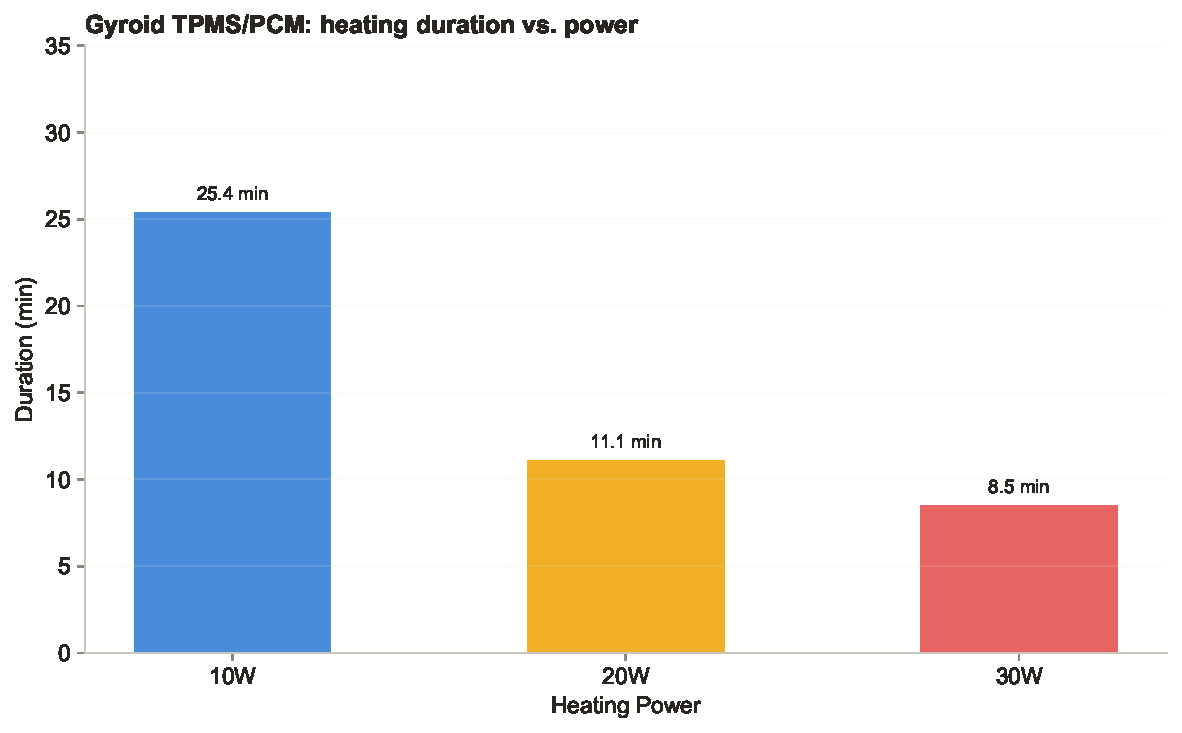
\includegraphics[width=0.7\linewidth]{figures/fig_03_duration.pdf}
\caption{Heating duration versus power for the Gyroid TPMS/PCM composite.}
\label{fig:duration}
\end{figure}

\paragraph{Outlier sensor analysis.}
The systematic identification of outlier sensors (Table~\ref{tab:outliers}) reveals spatially consistent patterns. $T_6$ was identified as an outlier in Group~C at both 10~W and 30~W, suggesting a position-dependent thermal anomaly---possibly due to imperfect thermal contact with the PCM or a slightly different local lattice geometry. The variation of the Group~B outlier ($T_3$ at 10/20~W vs.\ $T_5$ at 30~W) suggests that the thermal field within the intermediate region is sensitive to the heating rate, potentially reflecting different convection patterns in the molten PCM at different power levels~\cite{parida2020effect,cao2021characterization}.

\paragraph{Implications for TPMS-enhanced PCM.}
The results demonstrate that the AlSiMg Gyroid TPMS lattice provides effective thermal conductivity enhancement for the paraffin PCM. At 10~W, the temperature spread between the innermost and outermost sensor groups (17.1\textdegree C) is substantially smaller than what would be expected in a bare PCM system, where thermal gradients of 30--50\textdegree C are typical~\cite{souayfane2018melting}. The TPMS lattice acts as a distributed heat transfer network, conducting heat from the central heater radially outward through its high-conductivity metallic struts while the PCM absorbs and stores thermal energy through phase change.

The relatively small temperature difference between Groups B and C (10.6\textdegree C at 10~W, 2.1\textdegree C at 20~W, 15.2\textdegree C at 30~W) suggests that the TPMS lattice effectively homogenizes the temperature field in the outer region, which is advantageous for uniform thermal energy storage. The larger spread at 30~W may reflect the shorter experiment duration, which limits the time available for lateral heat conduction to establish thermal equilibrium.
